% UTF-8 encoding
% Compile with latex+dvipdfmx, pdflatex, xelatex or lualatex

\documentclass[UTF8]{ctexart}
\usepackage{graphicx}
\usepackage{amssymb}
\usepackage{amsmath}
\usepackage{subfigure}
\usepackage{geometry}
\usepackage{caption}

\newcommand{\true}{{\rm T}}
\newcommand{\false}{{\rm F}}
\newcommand{\snatural}{\mathbb{N}}
\newcommand{\sinteger}{\mathbb{Z}}
\newcommand{\srational}{\mathbb{Q}}
\newcommand{\sreal}{\mathbb{R}}
\newcommand{\card}{\rm{card}}
\newcommand{\modt}{\text{mod }}
\newcommand{\ran}{{\rm ran}}
\newcommand{\dom}{{\rm dom}}

\title{离散数学——第十三周作业}
\author{计83  刘轩奇  2018011025}
\date{2019.12.06}

\geometry{left=2.0cm, right=2.0cm, top=2.5cm, bottom=2.5cm}

\begin{document}

\maketitle

\paragraph{10.28} \label{10.28}
    对有限集合$A$,在$A$上给出最多个等价类和最少个等价类的关系各是什么?

\paragraph{答}
    给出最多个等价类的关系是恒等关系$I_A$,有$|A|$个等价类。给出最少个等价类的关系是全关系$E_A$,仅$1$个等价类。

\paragraph{10.29} \label{10.29}
    设$R$是$A$上传递和自反的关系,$T$是$A$上的关系,$aTb \Longleftrightarrow aRb \land bRa$。证明$T$是等价关系。

\paragraph{证}
    \begin{align*}
        R \text{是自反的} & \Longleftrightarrow ( \forall x)(x \in A \longrightarrow \langle x,x \rangle \in R) \\
        & \Longleftrightarrow ( \forall x)(x \in A \longrightarrow \langle x,x \rangle \in R \land \langle x,x \rangle \in R) \\
        & \Longleftrightarrow ( \forall x)( \langle x,x \rangle \in T)  \\
        & \Longleftrightarrow T \text{是自反的}
    \end{align*}

    $R$是对称的,则对任意$ \langle x,y \rangle $
    \begin{align*}
        \langle x,y \rangle \in T & \Longleftrightarrow \langle x,y \rangle \in R \land \langle y,x \rangle \in R \\
        & \Longleftrightarrow \langle y,x \rangle \in R \land \langle x,y \rangle \in R \\
        & \Longleftrightarrow \langle y,x \rangle \in T 
    \end{align*}
    从而$T$是对称的。

    $R$是传递的,则对任意$ \langle x,y \rangle, \langle y,z \rangle $
    \begin{align*}
        \langle x,y \rangle \in T \land \langle y,z \rangle \in T & \Longleftrightarrow \langle x,y \rangle \in R \land \langle y,x \rangle \in R \land \langle y,z \rangle \in R \land \langle z,y \rangle \in R \\
        & \Longrightarrow \langle x,z \rangle \in R \land \langle z,x \rangle \in R \\
        & \Longleftrightarrow \langle x,z \rangle \in T
    \end{align*}
    从而$T$是传递的。

    综上,$T$是等价关系。

\paragraph{10.30} \label{10.30}
    对$A= \{ a,b,c,d \} $,$R$是$A$上的等价关系,且
    $$R = \{ \langle a,a \rangle , \langle a,b \rangle , \langle b,a \rangle , \langle b,b \rangle , \langle c,c \rangle , \langle c,d \rangle , \langle d,c \rangle , \langle d,d \rangle \} $$
    画$R$的关系图,求$A$中各元素的等价类。

\paragraph{解}
    关系图如图10-30所示,等价类
    $$[a]_R = [b]_R = \{a,b\}$$
    $$[c]_R = [d]_R = \{c,d\}$$

    \begin{figure}[!htb]
        \centering
        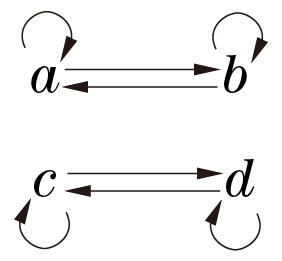
\includegraphics[width=0.188\textwidth]{10-30.png}
        \caption*{图 10-30}
    \end{figure}

\paragraph{10.31} \label{10.31}
    设$\sinteger_+= \{ x | x \in \sinteger \land x > 0 \} $,判定下列集合$\pi$是否构成$\sinteger_+$的划分。
    
    (1) $S_1 = \{ x| x \in \sinteger_+ \land x \text{是素数} \}, S_2 = \sinteger_+ - S_1, \pi = \{S_1, S_2 \} $

    (2) $\pi = \{ \{ x \} |x \in \sinteger_+ \} $

\paragraph{答}
    (1) 是,$\pi$划分将$\sinteger_+$划分为素数与非素数。

    (2) 是,$\pi$划分即是恒等关系导出的划分。

\paragraph{10.32} \label{10.32}
    对非空集合$A$,$P(A) - \{\varnothing\}$是否构成$A$的划分?

\paragraph{答}
    若$|A|=1$,则$P(A) - \{\varnothing\} = \{A\}$是$A$的划分,等同于全关系导出的划分。

    若$|A|>1$,则$P(A) - \{\varnothing\}$不是$A$的划分,因为$P(A) - \{\varnothing\}$的元素$A$和$\{a\}$(其中$a$为$A$的任意元素)交集不为空。
    
\paragraph{10.33} \label{10.33}
    有$4$个元素的集合上,不同的等价关系的数目是多少?

\paragraph{答}
    不同等价关系的数目等同于不同划分的数目,而不同的划分有(1)恒等关系导出的划分;(2)二一一型划分;(3)二二型划分;(4)三一型划分;(5)全关系导出的划分,共15种,如下所示。则不同等价关系的数目亦为15。

    $ (1) \{ \{ a \} , \{ b \} , \{ c \} , \{ d \} \} $

    $ (2) \{ \{ a,b \} , \{ c \} , \{ d \} \} , \{ \{ a,c \} , \{ b \} , \{ d \} \} , \{ \{ a,d \} , \{ b \} , \{ c \} \} ,$ 

    \quad \quad $ \{ \{ b,c \} , \{ a \} , \{ d \} \} , \{ \{ b,d \} , \{ a \} , \{ c \} \} , \{ \{ c,d \} , \{ a \} , \{ b \} \} $

    $ (3) \{ \{ a,b \} , \{ c,d \} \} , \{ \{ a,c \} , \{ b,d \} \} , \{ \{ a,d \} , \{ b,c \} \} $

    $ (4) \{ \{ a,b,c \} , \{ d \} \} , \{ \{ a,b,d \} , \{ c \} \} , \{ \{ a,c,d \} , \{ b \} \} , \{ \{ b,c,d \} , \{ a \} \} $

    $ (5) \{ \{ a,b,c,d \} \} $

\paragraph{10.34} \label{10.34}
    设$R,S$是$A$上的关系,且
    $$S = \{ \langle a,b \rangle | ( \exists c) (aRc \land cRb) \} $$
    证明若$R$是等价关系,则$S$是等价关系。

\paragraph{证}
    $R$是等价关系,则$R$自反、对称且传递。
    \begin{align*}
        a \in A & \Longrightarrow \langle a,a \rangle \in R \\
        & \Longleftrightarrow \langle a,a \rangle \in R \land \langle a,a \rangle \in R \\
        & \Longleftrightarrow \langle a,a \rangle \in S
    \end{align*}
    则$S$自反。
    \begin{align*}
        \langle a,b \rangle \in S & \Longleftrightarrow ( \exists c)(aRc \land cRb) \\
        & \Longrightarrow ( \exists c)(cRa \land bRc) \\
        & \Longleftrightarrow \langle b,a \rangle \in S
    \end{align*}
    则$S$对称。
    \begin{align*}
        \langle a,b \rangle \in S \land \langle b,c \rangle \in S & \Longleftrightarrow ( \exists d)(aRd \land dRb) \land ( \exists e)(bRe \land eRc) \\
        & \Longleftrightarrow ( \exists d) ( \exists e)(aRd \land dRb \land bRe \land eRc) \\
        & \Longrightarrow ( \exists d) ( \exists e)(aRd \land dRe \land eRc) \\
        & \Longrightarrow ( \exists d)(a Rd \land dRc) \\
        & \Longleftrightarrow \langle a,c \rangle \in S
    \end{align*}
    则$S$传递。
    
    综上,$S$是等价关系。

\paragraph{10.35} \label{10.35}
    设$\sinteger_+$是正整数集合,$A = \sinteger_+ \times \sinteger_+$,$A$上的关系
    $$R= \{ \langle \langle x,y \rangle , \langle u,v \rangle \rangle | xv = yu \} $$
    证明$R$是等价关系。

\paragraph{证}
    $$ \langle x,y \rangle \in A \Longleftrightarrow xy = xy \Longleftrightarrow \langle \langle x,y \rangle , \langle x,y \rangle \rangle \in R$$
    则$R$自反。
    \begin{align*}
        \langle \langle x,y \rangle , \langle u,v \rangle \rangle \in R & \Longleftrightarrow xy = uv \\
        & \Longleftrightarrow \langle \langle u,v \rangle , \langle x,y \rangle \rangle \in R
    \end{align*}
    则$R$对称。
    \begin{align*}
        \langle \langle x,y \rangle , \langle u,v \rangle \rangle \in R \land \langle \langle u,v \rangle , \langle z,w \rangle \rangle \in R & \Longleftrightarrow xy = uv \land uv = zw \\
        & \Longrightarrow xy = zw \\
        & \Longrightarrow \langle \langle x,y \rangle , \langle z,w \rangle \rangle \in R
    \end{align*}
    则$R$传递。

    综上,$R$是等价关系。

\paragraph{10.39} \label{10.39}
    对下列集合上的整除关系,画出Hasse图。
    
    (1) \{1,2,3,4,6,8,12,24\}

    (2) \{1,2,3,4,5,6,7,8,9\}

\paragraph{答}
    如图10-39所示。

    \begin{figure}[!htb]
        \centering
        \begin{minipage}[t]{0.153\textwidth}
        \centering
        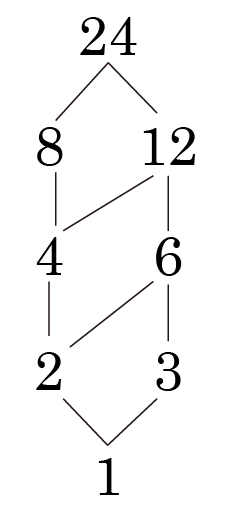
\includegraphics[width=1\textwidth]{10-39-1.png}
        \caption*{(1)}
        \end{minipage}
        \begin{minipage}[t]{0.259\textwidth}
        \centering
        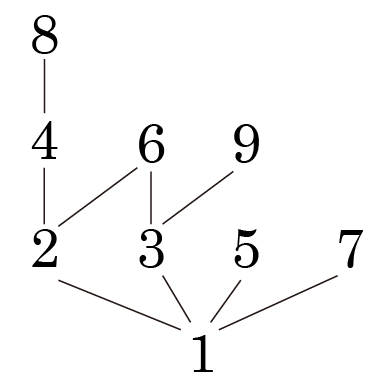
\includegraphics[width=1\textwidth]{10-39-2.png}
        \caption*{(2)}
        \end{minipage}
        \caption*{图 10-39}
    \end{figure}

\paragraph{10.40} \label{10.40}
    写出下列Hasse图(图10-40)的集合和集合上的偏序关系。

    \begin{figure}[!htb]
        \centering
        \begin{minipage}[t]{0.241\textwidth}
        \centering
        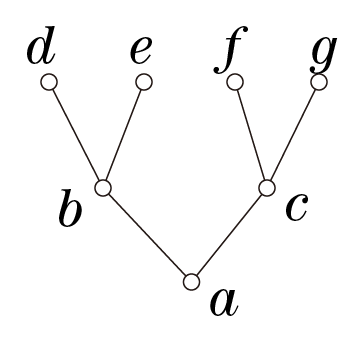
\includegraphics[width=1\textwidth]{10-40-a.png}
        \caption*{(a)}
        \end{minipage}
        \begin{minipage}[t]{0.230\textwidth}
        \centering
        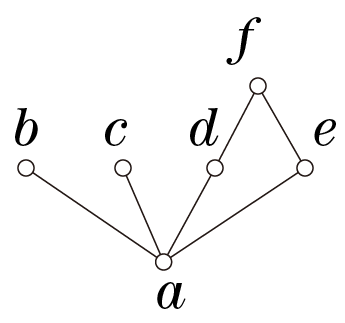
\includegraphics[width=1\textwidth]{10-40-b.png}
        \caption*{(b)}
        \end{minipage}
        \caption*{图 10-40}
    \end{figure}

\paragraph{答}
    (1) 
    $$A = \{ a,b,c,d,e,f,g \} $$
    \begin{align*}
        R = & \{ \langle a,a \rangle , \langle a,b \rangle , \langle a,c \rangle , \langle a,d \rangle , \langle a,e \rangle , \langle a,f \rangle , \langle a,g \rangle , \\
        & \langle b,b \rangle , \langle b,d \rangle , \langle b,e \rangle , \langle c,c \rangle , \langle c,f \rangle , \langle c,g \rangle , \\
        & \langle d,d \rangle , \langle e,e \rangle , \langle f,f \rangle , \langle g,g \rangle \} 
    \end{align*}

    (2)
    $$A = \{ a,b,c,d,e,f \} $$
    \begin{align*}
        R = & \{ \langle a,a \rangle , \langle a,b \rangle , \langle a,c \rangle , \langle a,d \rangle , \langle a,e \rangle , \langle a,f \rangle , \\
        & \langle b,b \rangle , \langle c,c \rangle , \langle d,d \rangle , \langle d,f \rangle , \langle e,e \rangle , \langle e,f \rangle , \langle f,f \rangle \}
    \end{align*}

\paragraph{10.41} \label{10.41}
    画出下列偏序集$ \langle A,R \rangle $的Hasse图,并写出$A$的极大元、极小元、最大元、最小元。

    (1) $$A = \{ a,b,c,d,e \} , R= \{ \langle a,d \rangle , \langle a,c \rangle , \langle a,b \rangle , \langle a,e \rangle , \langle b,e \rangle , \langle c,e \rangle , \langle d,e \rangle \} \cup I_A $$

    (2) $$A = \{ a,b,c,d \} , R = \{ \langle c,d \rangle \} \cup I_A$$

\paragraph{答}
    Hasse图如图10-41所示。
    
    (1) 极大元:$e$;极小元:$a$;最大元:$e$;最小元:$a$。

    (2) 极大元:$a,b,d$;极小元:$a,b,c$;无最大、最小元。

    \begin{figure}[!htb]
        \centering
        \begin{minipage}[t]{0.211\textwidth}
        \centering
        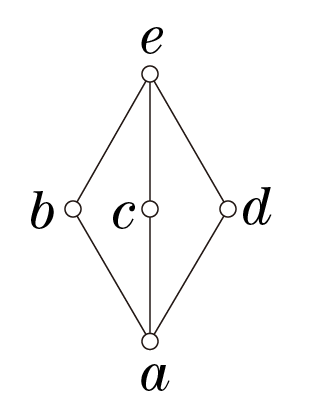
\includegraphics[width=1\textwidth]{10-41-1.png}
        \caption*{(1)}
        \end{minipage}
        \begin{minipage}[t]{0.183\textwidth}
        \centering
        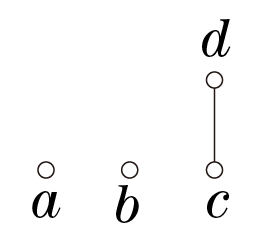
\includegraphics[width=1\textwidth]{10-41-2.png}
        \caption*{(2)}
        \end{minipage}
        \caption*{图 10-41}
    \end{figure}

\paragraph{10.42} \label{10.42}
    设$\sinteger_+= \{ x| x \in \sinteger \land x \rangle 0 \} $,$D$是$\sinteger_+$上的整除关系,$T = \{ 1,2, \cdots, 10 \} \subseteq \sinteger_+$。在偏序集$ \langle \sinteger_+, D \rangle $中,求$T$的上界、下界、上确界、下确界。
    
\paragraph{解}
    $T$的下界、下确界均为$1$;$T$的上界$k$是$T$中所有数字的倍数,则$k = n{\rm LCM}\{1,2,3,4,5,6,7,8,9,10\}=2520n(n \in \sinteger_+)$,其中${\rm LCM}$表示最小公倍数,$T$的上确界即$2520$。
    
\paragraph{10.43} \label{10.43}
    设$R$是$A$上的偏序关系,$B\subseteq A$,证明$R \cap (B \times B)$是$B$上的偏序关系。

\paragraph{证}
    记$B \times B = E_B$是$B$上的全关系。
    $$r(R \cap (B \times B)) \upharpoonright_B = r(R) \upharpoonright_B = R \cap (B \times B)$$
    则$R \cap (B \times B)$自反。

    $a \neq b$时,
    \begin{align*}
        \langle a,b \rangle \in R \cap (B \times B) & \Longleftrightarrow \langle a,b \rangle \in R \land \langle a,b \rangle \in E_B \\
        & \Longrightarrow \langle b,a \rangle \notin R \\
        & \Longrightarrow \langle b,a \rangle \notin R \cap (B \times B) 
    \end{align*}
    则$R \cap (B \times B)$反对称。
    \begin{align*}
        \langle a,b \rangle , \langle b,c \rangle \in R \cap (B \times B) & \Longrightarrow \langle a,b \rangle \in R \land \langle b,c \rangle \in R \\
        & \Longrightarrow \langle a,c \rangle \in R \\
        & \Longrightarrow \langle a,c \rangle \in R \cap (B \times B) 
    \end{align*}    
    则$R \cap (B \times B)$传递。

    综上,$R \cap (B \times B)$是$B$上的偏序关系。

\paragraph{10.45} \label{10.45}
    给出$A=\{0,1,2\}$上所有的偏序关系的Hasse图。

\paragraph{解}
    如图10-45所示,共19种关系。

    \begin{figure}[!htb]
        \centering
        \begin{minipage}[t]{0.111\textwidth}
        \centering
        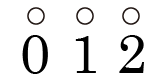
\includegraphics[width=1\textwidth]{10-45-a.png}
        \caption*{(a) 空关系的Hasse图}
        \end{minipage}
        \\
        \begin{minipage}[t]{0.532\textwidth}
        \centering
        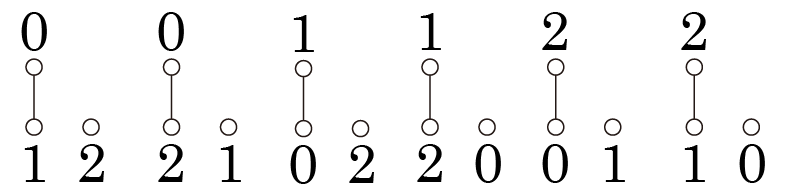
\includegraphics[width=1\textwidth]{10-45-b.png}
        \caption*{(b) 含一条边的Hasse图}
        \end{minipage}
        \\
        \begin{minipage}[t]{0.507\textwidth}
        \centering
        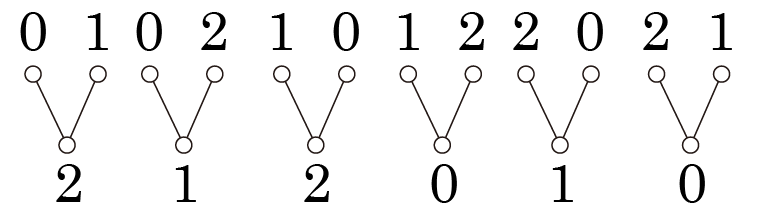
\includegraphics[width=1\textwidth]{10-45-c.png}
        \caption*{(c) 含两条边的V形Hasse图}
        \end{minipage}
        \\
        \begin{minipage}[t]{0.513\textwidth}
        \centering
        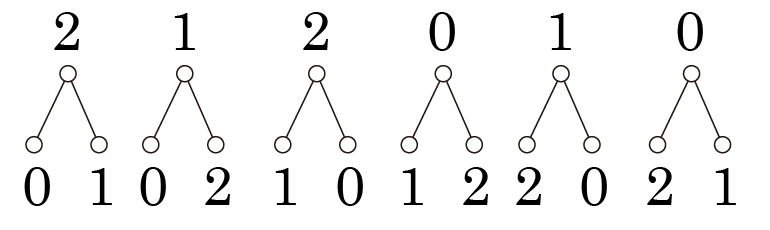
\includegraphics[width=1\textwidth]{10-45-d.png}
        \caption*{(d) 含两条边的$\Lambda$形Hasse图}
        \end{minipage}
        \\
        \begin{minipage}[t]{0.384\textwidth}
        \centering
        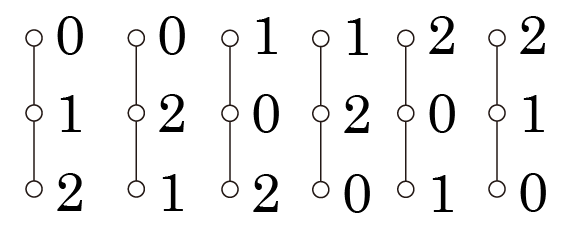
\includegraphics[width=1\textwidth]{10-45-e.png}
        \caption*{(e) 单链形Hasse图}
        \end{minipage}
        \caption*{图 10-45}
    \end{figure}

\end{document} 